%%%%%%%%%%%%%%%%%%%%%%%%%%%%%%%%%%%%%%%%%%%%%%%%%%%%%%%%%%%%%%%%%%%%%%%%%%%%%%%
% Chapter 'Refrigerants - CarbonDioxide'
%%%%%%%%%%%%%%%%%%%%%%%%%%%%%%%%%%%%%%%%%%%%%%%%%%%%%%%%%%%%%%%%%%%%%%%%%%%%%%%
\section{CarbonDioxide}
%
%%%%%%%%%%%%%%%%%%%%%%%%%%%%%%%%%%%%%%%%%%%%%%%%%%%%%%%%%%%%%%%%%%%%%%%%%%%%%%%
%%%%%%%%%%%%%%%%%%%%%%%%%%%%%%%%%%%%%%%%%%%%%%%%%%%%%%%%%%%%%%%%%%%%%%%%%%%%%%%
\subsection{Saturated Liquid Density - EoS1 - ID 1}
%
\begin{tabular}[l]{|lp{11.5cm}|}
\hline
\addlinespace

\textbf{Name:} & CarbonDioxide \\
\textbf{Equation:} & SaturatedLiquidDensity\_EoS1 \\
\textbf{ID:} & 1 \\
\textbf{Reference:} & Span, Roland; Wagner, Wolfgang (1996): A New Equation of State for Carbon Dioxide Covering the Fluid Region from the Triple‐Point Temperature to 1100 K at Pressures up to 800 MPa. In: Journal of Physical and Chemical Reference Data 25 (6), S. 1509–1596. DOI: 10.1063/1.555991. \\
\textbf{Comment:} & None \\

\addlinespace
\hline
\end{tabular}
\newline

\textbf{Equation and parameters:}
\newline
%
Saturated liquid density $\rho_\mathrm{sat}^\mathrm{liq}$ in $\si{\kilogram\per\cubic\meter}$ is calculated depending on temperature $T$ in $\si{\kelvin}$ by:
%
\begin{equation*}
\begin{split}
\rho_\mathrm{sat}^\mathrm{liq} &=& \begin{cases} \rho_\mathrm{ref} \exp(\Omega) & \quad \text{if flag } < 0 \\ \rho_\mathrm{ref} \Omega & \quad \text{else} \end{cases} & \quad\text{, with} \\
\Omega &=& \sum_{i=1}^{8} a_i \xi^{b_i} & \quad\text{, and} \\
\xi &=& 1 - \theta & \quad\text{, and} \\
\theta &=& \nicefrac{T}{T_\mathrm{crit}} & \quad\text{.}
\end{split}
\end{equation*}
%
The parameters of the equation are:
%
\begin{longtable}[l]{lll|lll}
\toprule
\addlinespace
\textbf{Par.} & \textbf{Unit} & \textbf{Value} &	\textbf{Par.} & \textbf{Unit} & \textbf{Value} \\
\addlinespace
\midrule
\endhead

\bottomrule
\endfoot
\bottomrule
\endlastfoot
\addlinespace

flag & - & -1.000000000e+00 & $b_4$ & - & 1.833333333e+00 \\
$T_\mathrm{crit}$ & $\si{\kelvin}$ & 3.041282000e+02 & $a_5$ & - & 0.000000000e+00 \\
$\rho_\mathrm{ref}$ & $\si{\kilogram\per\cubic\meter}$ & 4.676000000e+02 & $b_5$ & - & 0.000000000e+00 \\
$a_1$ & - & 1.924510800e+00 & $a_6$ & - & 0.000000000e+00 \\
$b_1$ & - & 3.400000000e-01 & $b_6$ & - & 0.000000000e+00 \\
$a_2$ & - & -6.238555500e-01 & $a_7$ & - & 0.000000000e+00 \\
$b_2$ & - & 5.000000000e-01 & $b_7$ & - & 0.000000000e+00 \\
$a_3$ & - & -3.273112700e-01 & $a_8$ & - & 0.000000000e+00 \\
$b_3$ & - & 1.666666667e+00 & $b_8$ & - & 0.000000000e+00 \\
$a_4$ & - & 3.924514200e-01 & & & \\

\addlinespace\end{longtable}

\textbf{Validity:}
\newline
Equation is approximately valid for $216.59 \si{\kelvin} \leq T \leq 304.1282 \si{\kelvin}$.
\newline

\textbf{Visualization:}
%
\begin{figure}[!htp]
{\noindent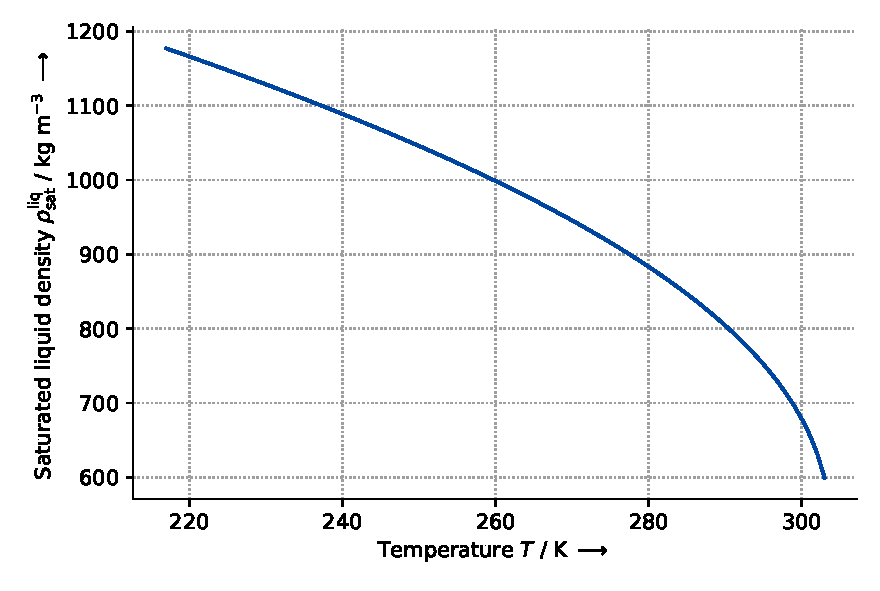
\includegraphics[height=10cm, keepaspectratio]{figs/ref/ref_CarbonDioxide_SaturatedLiquidDensity_EoS1_1.pdf}}
\end{figure}
%

\FloatBarrier
\newpage
%%%%%%%%%%%%%%%%%%%%%%%%%%%%%%%%%%%%%%%%%%%%%%%%%%%%%%%%%%%%%%%%%%%%%%%%%%%%%%%
%%%%%%%%%%%%%%%%%%%%%%%%%%%%%%%%%%%%%%%%%%%%%%%%%%%%%%%%%%%%%%%%%%%%%%%%%%%%%%%
\subsection{Saturated Liquid Density - EoS1 - ID 2}
%
\begin{tabular}[l]{|lp{11.5cm}|}
\hline
\addlinespace

\textbf{Name:} & CarbonDioxide \\
\textbf{Equation:} & SaturatedLiquidDensity\_EoS1 \\
\textbf{ID:} & 2 \\
\textbf{Reference:} & Verein Deutscher Ingenieure (2010): VDI Heat Atlas. 2. Ed. Heidelberg: Springer. Online: http://dx.doi.org/10.1007/978-3-540-77877-6. \\
\textbf{Comment:} & None \\

\addlinespace
\hline
\end{tabular}
\newline

\textbf{Equation and parameters:}
\newline
%
Saturated liquid density $\rho_\mathrm{sat}^\mathrm{liq}$ in $\si{\kilogram\per\cubic\meter}$ is calculated depending on temperature $T$ in $\si{\kelvin}$ by:
%
\begin{equation*}
\begin{split}
\rho_\mathrm{sat}^\mathrm{liq} &=& \begin{cases} \rho_\mathrm{ref} \exp(\Omega) & \quad \text{if flag } < 0 \\ \rho_\mathrm{ref} \Omega & \quad \text{else} \end{cases} & \quad\text{, with} \\
\Omega &=& \sum_{i=1}^{8} a_i \xi^{b_i} & \quad\text{, and} \\
\xi &=& 1 - \theta & \quad\text{, and} \\
\theta &=& \nicefrac{T}{T_\mathrm{crit}} & \quad\text{.}
\end{split}
\end{equation*}
%
The parameters of the equation are:
%
\begin{longtable}[l]{lll|lll}
\toprule
\addlinespace
\textbf{Par.} & \textbf{Unit} & \textbf{Value} &	\textbf{Par.} & \textbf{Unit} & \textbf{Value} \\
\addlinespace
\midrule
\endhead

\bottomrule
\endfoot
\bottomrule
\endlastfoot
\addlinespace

flag & - & 1.000000000e+00 & $b_4$ & - & 1.000000000e+00 \\
$T_\mathrm{crit}$ & $\si{\kelvin}$ & 3.041300000e+02 & $a_5$ & - & 8.102948718e-02 \\
$\rho_\mathrm{ref}$ & $\si{\kilogram\per\cubic\meter}$ & 4.680000000e+02 & $b_5$ & - & 1.333333333e+00 \\
$a_1$ & - & 1.000000000e+00 & $a_6$ & - & 0.000000000e+00 \\
$b_1$ & - & 0.000000000e+00 & $b_6$ & - & 0.000000000e+00 \\
$a_2$ & - & 1.918531410e+00 & $a_7$ & - & 0.000000000e+00 \\
$b_2$ & - & 3.500000000e-01 & $b_7$ & - & 0.000000000e+00 \\
$a_3$ & - & 3.633354701e-01 & $a_8$ & - & 0.000000000e+00 \\
$b_3$ & - & 6.666666667e-01 & $b_8$ & - & 0.000000000e+00 \\
$a_4$ & - & 3.612213675e-01 & & & \\

\addlinespace\end{longtable}

\textbf{Validity:}
\newline
Equation is approximately valid for $216.59 \si{\kelvin} \leq T \leq 304.13 \si{\kelvin}$.
\newline

\textbf{Visualization:}
%
\begin{figure}[!htp]
{\noindent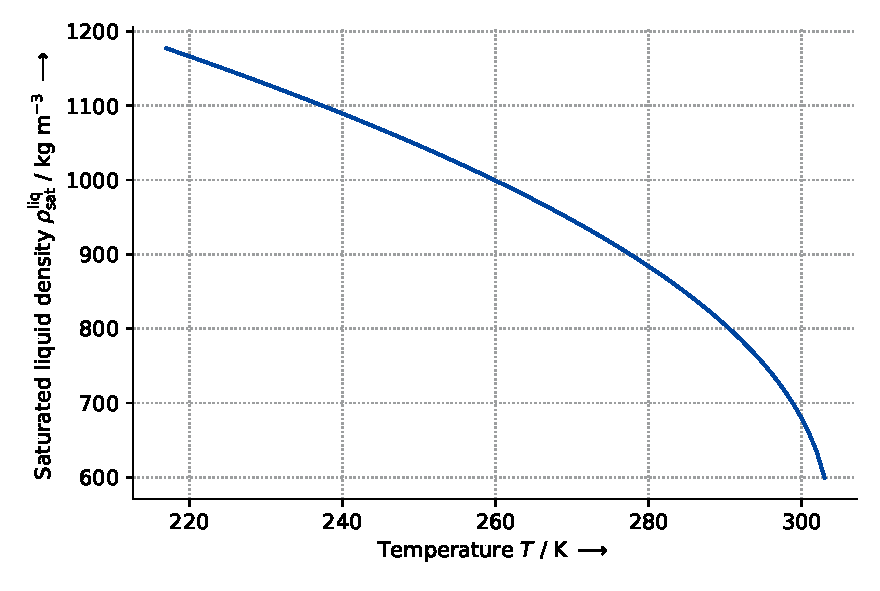
\includegraphics[height=10cm, keepaspectratio]{figs/ref/ref_CarbonDioxide_SaturatedLiquidDensity_EoS1_2.pdf}}
\end{figure}
%

\FloatBarrier
\newpage
%%%%%%%%%%%%%%%%%%%%%%%%%%%%%%%%%%%%%%%%%%%%%%%%%%%%%%%%%%%%%%%%%%%%%%%%%%%%%%%
%%%%%%%%%%%%%%%%%%%%%%%%%%%%%%%%%%%%%%%%%%%%%%%%%%%%%%%%%%%%%%%%%%%%%%%%%%%%%%%
\subsection{Vapor Pressure - Antoine - ID 1}
%
\begin{tabular}[l]{|lp{11.5cm}|}
\hline
\addlinespace

\textbf{Name:} & CarbonDioxide \\
\textbf{Equation:} & VaporPressure\_Antoine \\
\textbf{ID:} & 1 \\
\textbf{Reference:} & P.J. Linstrom and W.G. Mallard, Eds., NIST Chemistry WebBook, NIST Standard Reference Database Number 69, National Institute of Standards and Technology, Gaithersburg MD, 20899, https://doi.org/10.18434/T4D303. \\
\textbf{Comment:} & None \\

\addlinespace
\hline
\end{tabular}
\newline

\textbf{Equation and parameters:}
\newline
%
Vapor pressure $p_\mathrm{sat}$ in $\si{\pascal}$ is calculated depending on temperature $T$ in $\si{\kelvin}$ by:
%
\begin{equation*}
\nicefrac{p_\mathrm{sat}}{100000} = 10^{a - \nicefrac{b}{T + c}}
\end{equation*}
%
The parameters of the equation are:
%
\begin{longtable}[l]{lll|lll}
\toprule
\addlinespace
\textbf{Par.} & \textbf{Unit} & \textbf{Value} &	\textbf{Par.} & \textbf{Unit} & \textbf{Value} \\
\addlinespace
\midrule
\endhead

\bottomrule
\endfoot
\bottomrule
\endlastfoot
\addlinespace

$a$ & - & 6.812280000e+00 & $c$ & $\si{\kelvin}$  & -3.494000000e+00 \\
$b$ & $\si{\kelvin}$ & 1.301679000e+03 & & & \\

\addlinespace\end{longtable}

\textbf{Validity:}
\newline
Equation is approximately valid for $154.26 \si{\kelvin} \leq T \leq 195.89 \si{\kelvin}$.
\newline

\textbf{Visualization:}
%
\begin{figure}[!htp]
{\noindent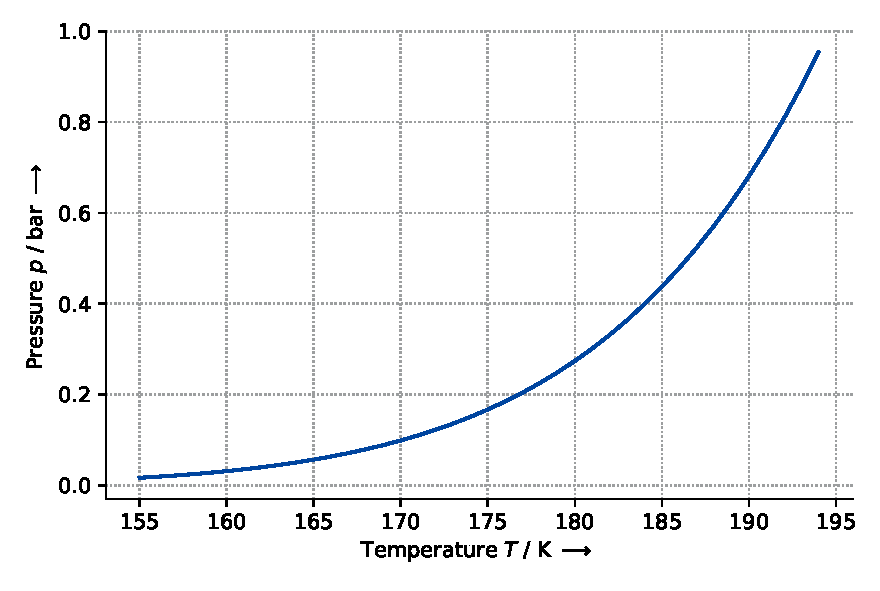
\includegraphics[height=10cm, keepaspectratio]{figs/ref/ref_CarbonDioxide_VaporPressure_Antoine_1.pdf}}
\end{figure}
%

\FloatBarrier
\newpage
%%%%%%%%%%%%%%%%%%%%%%%%%%%%%%%%%%%%%%%%%%%%%%%%%%%%%%%%%%%%%%%%%%%%%%%%%%%%%%%
%%%%%%%%%%%%%%%%%%%%%%%%%%%%%%%%%%%%%%%%%%%%%%%%%%%%%%%%%%%%%%%%%%%%%%%%%%%%%%%
\subsection{Vapor Pressure - EoS1 - ID 1}
%
\begin{tabular}[l]{|lp{11.5cm}|}
\hline
\addlinespace

\textbf{Name:} & CarbonDioxide \\
\textbf{Equation:} & VaporPressure\_EoS1 \\
\textbf{ID:} & 1 \\
\textbf{Reference:} & Span, Roland; Wagner, Wolfgang (1996): A New Equation of State for Carbon Dioxide Covering the Fluid Region from the Triple‐Point Temperature to 1100 K at Pressures up to 800 MPa. In: Journal of Physical and Chemical Reference Data 25 (6), S. 1509–1596. DOI: 10.1063/1.555991. \\
\textbf{Comment:} & None \\

\addlinespace
\hline
\end{tabular}
\newline

\textbf{Equation and parameters:}
\newline
%
Vapor pressure $p_\mathrm{sat}$ in $\si{\pascal}$ is calculated depending on temperature $T$ in $\si{\kelvin}$ by:
%
\begin{equation*}
\begin{split}
p_\mathrm{sat} &=& p_\mathrm{crit} \exp \left( \nicefrac{1}{\theta} \sum_{i=1}^{7} a_i \xi^{b_i} \right) & \quad\text{, and} \\
\xi &=& 1 - \theta & \quad\text{, and} \\
\theta &=& \nicefrac{T}{T_\mathrm{crit}} & \quad\text{.}
\end{split}
\end{equation*}
%
The parameters of the equation are:
%
\begin{longtable}[l]{lll|lll}
\toprule
\addlinespace
\textbf{Par.} & \textbf{Unit} & \textbf{Value} &	\textbf{Par.} & \textbf{Unit} & \textbf{Value} \\
\addlinespace
\midrule
\endhead

\bottomrule
\endfoot
\bottomrule
\endlastfoot
\addlinespace

$T_\mathrm{crit}$ & $\si{\kelvin}$ & 3.041282000e+02 & $a_4$ & - & -3.299563400e+00 \\
$p_\mathrm{crit}$ & $\si{\pascal}$ & 7.377300000e+06 & $b_4$ & - & 4.000000000e+00 \\
$a_1$ & - & -7.060208700e+00 & $a_5$ & - & 0.000000000e+00 \\
$b_1$ & - & 1.000000000e+00 & $b_5$ & - & 0.000000000e+00 \\
$a_2$ & - & 1.939121800e+00 & $a_6$ & - & 0.000000000e+00 \\
$b_2$ & - & 1.500000000e+00 & $b_6$ & - & 0.000000000e+00 \\
$a_3$ & - & -1.646359700e+00 & $a_7$ & - & 0.000000000e+00 \\
$b_3$ & - & 2.000000000e+00 & $b_7$ & - & 0.000000000e+00 \\

\addlinespace\end{longtable}

\textbf{Validity:}
\newline
Equation is approximately valid for $216.59 \si{\kelvin} \leq T \leq 304.1282 \si{\kelvin}$.
\newline

\textbf{Visualization:}
%
\begin{figure}[!htp]
{\noindent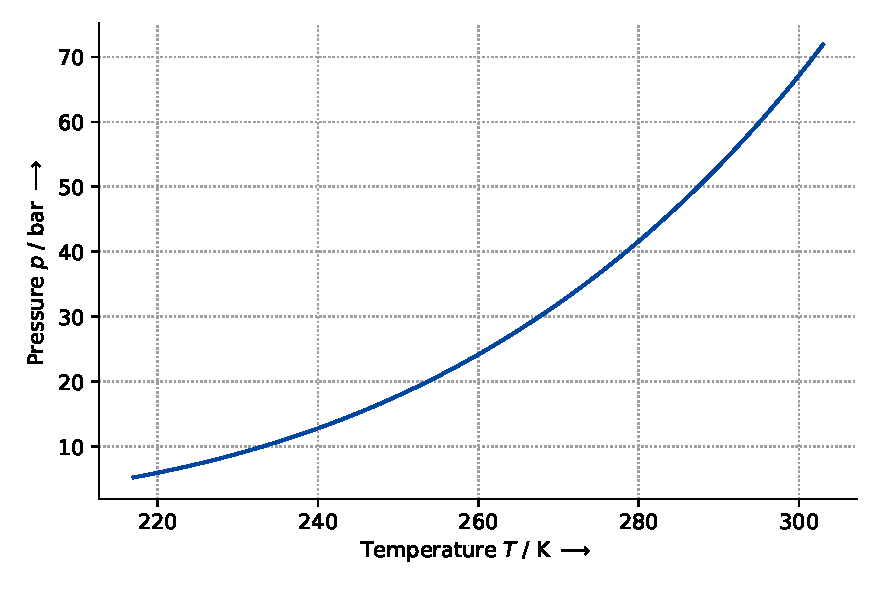
\includegraphics[height=10cm, keepaspectratio]{figs/ref/ref_CarbonDioxide_VaporPressure_EoS1_1.pdf}}
\end{figure}
%

\FloatBarrier
\newpage
%%%%%%%%%%%%%%%%%%%%%%%%%%%%%%%%%%%%%%%%%%%%%%%%%%%%%%%%%%%%%%%%%%%%%%%%%%%%%%%
%%%%%%%%%%%%%%%%%%%%%%%%%%%%%%%%%%%%%%%%%%%%%%%%%%%%%%%%%%%%%%%%%%%%%%%%%%%%%%%
\subsection{Vapor Pressure - EoS1 - ID 2}
%
\begin{tabular}[l]{|lp{11.5cm}|}
\hline
\addlinespace

\textbf{Name:} & CarbonDioxide \\
\textbf{Equation:} & VaporPressure\_EoS1 \\
\textbf{ID:} & 2 \\
\textbf{Reference:} & Verein Deutscher Ingenieure (2010): VDI Heat Atlas. 2. Ed. Heidelberg: Springer. Online: http://dx.doi.org/10.1007/978-3-540-77877-6. \\
\textbf{Comment:} & None \\

\addlinespace
\hline
\end{tabular}
\newline

\textbf{Equation and parameters:}
\newline
%
Vapor pressure $p_\mathrm{sat}$ in $\si{\pascal}$ is calculated depending on temperature $T$ in $\si{\kelvin}$ by:
%
\begin{equation*}
\begin{split}
p_\mathrm{sat} &=& p_\mathrm{crit} \exp \left( \nicefrac{1}{\theta} \sum_{i=1}^{7} a_i \xi^{b_i} \right) & \quad\text{, and} \\
\xi &=& 1 - \theta & \quad\text{, and} \\
\theta &=& \nicefrac{T}{T_\mathrm{crit}} & \quad\text{.}
\end{split}
\end{equation*}
%
The parameters of the equation are:
%
\begin{longtable}[l]{lll|lll}
\toprule
\addlinespace
\textbf{Par.} & \textbf{Unit} & \textbf{Value} &	\textbf{Par.} & \textbf{Unit} & \textbf{Value} \\
\addlinespace
\midrule
\endhead

\bottomrule
\endfoot
\bottomrule
\endlastfoot
\addlinespace

$T_\mathrm{crit}$ & $\si{\kelvin}$ & 3.041300000e+02 & $a_4$ & - & -2.348530000e+00 \\
$p_\mathrm{crit}$ & $\si{\pascal}$ & 7.377000000e+06 & $b_4$ & - & 5.000000000e+00 \\
$a_1$ & - & -7.029160000e+00 & $a_5$ & - & 0.000000000e+00 \\
$b_1$ & - & 1.000000000e+00 & $b_5$ & - & 0.000000000e+00 \\
$a_2$ & - & 1.539370000e+00 & $a_6$ & - & 0.000000000e+00 \\
$b_2$ & - & 1.500000000e+00 & $b_6$ & - & 0.000000000e+00 \\
$a_3$ & - & -2.283300000e+00 & $a_7$ & - & 0.000000000e+00 \\
$b_3$ & - & 2.500000000e+00 & $b_7$ & - & 0.000000000e+00 \\

\addlinespace\end{longtable}

\textbf{Validity:}
\newline
Equation is approximately valid for $216.59 \si{\kelvin} \leq T \leq 304.13 \si{\kelvin}$.
\newline

\textbf{Visualization:}
%
\begin{figure}[!htp]
{\noindent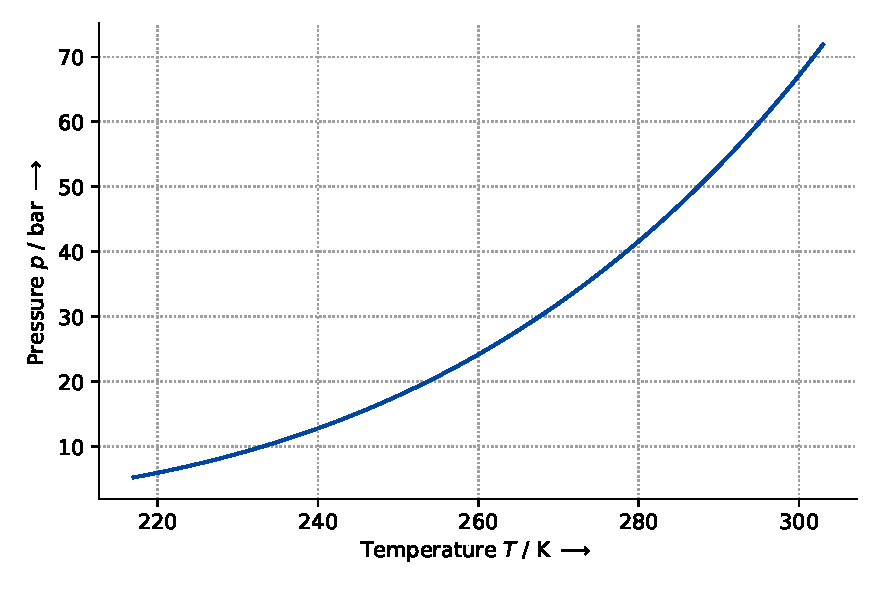
\includegraphics[height=10cm, keepaspectratio]{figs/ref/ref_CarbonDioxide_VaporPressure_EoS1_2.pdf}}
\end{figure}
%

\FloatBarrier
\newpage
%%%%%%%%%%%%%%%%%%%%%%%%%%%%%%%%%%%%%%%%%%%%%%%%%%%%%%%%%%%%%%%%%%%%%%%%%%%%%%%
%%%%%%%%%%%%%%%%%%%%%%%%%%%%%%%%%%%%%%%%%%%%%%%%%%%%%%%%%%%%%%%%%%%%%%%%%%%%%%%
\subsection{Vapor Pressure - EoSCubic - ID 1}
%
\begin{tabular}[l]{|lp{11.5cm}|}
\hline
\addlinespace

\textbf{Name:} & CarbonDioxide \\
\textbf{Equation:} & VaporPressure\_EoSCubic \\
\textbf{ID:} & 1 \\
\textbf{Reference:} & Lemmon, E. W.; Bell, I. H.; Huber, M. L.; McLinden, M. O. (2018): NIST Standard Reference Database 23. Reference Fluid Thermodynamic and Transport Properties-REFPROP, Version 10.0, National Institute of Standards and Technology. Online: https://www.nist.gov/srd/refprop. \\
\textbf{Comment:} & None \\

\addlinespace
\hline
\end{tabular}
\newline

\textbf{Equation and parameters:}
\newline
%
Vapor pressure $p_\mathrm{sat}$ in $\si{\pascal}$ is calculated depending on temperature $T$ in $\si{\kelvin}$ and molar volume v in $\si{\mole\per\cubic\meter}$ by using cubic equation of state. For this purpose, molar volumes of liquid and vapor phase are changed iteratively until fugacity coefficients of vapor and liquid phase are equal. Cubic equation of state is given by:
\begin{equation*}
\begin{split}
p &=& R \frac{T}{v - b} - \frac{a}{v \left(v + b\right)} & \quad\text{, and} \\
a &=& \frac{1}{9 \left(2^{\nicefrac{1}{3}} - 1\right)} \frac{\left(R T_\mathrm{crit} \right)^2}{p_\mathrm{crit}} \alpha & \quad\text{, and} \\
b &=& 0.08664 R \frac{T_\mathrm{crit}}{p_\mathrm{crit}} & \quad\text{, and} \\
\alpha &=& \left(1 + \kappa \left(1 - \sqrt(\nicefrac{T}{T_\mathrm{crit}}) \right) \right)^2 & \quad\text{, and} \\
\kappa &=& 0.48508 + 1.55171 \omega - 0.15613 \omega^2 & \quad\text{.}
\end{split}
\end{equation*}
%
The parameters of the equation are:
%
\begin{longtable}[l]{lll|lll}
\toprule
\addlinespace
\textbf{Par.} & \textbf{Unit} & \textbf{Value} &	\textbf{Par.} & \textbf{Unit} & \textbf{Value} \\
\addlinespace
\midrule
\endhead

\bottomrule
\endfoot
\bottomrule
\endlastfoot
\addlinespace

EoS & - & -5.000000000e+00 & $\beta_0$ & - & 0.000000000e+00 \\
$T_\mathrm{crit}$ & $\si{\kelvin}$ & 3.041300000e+02 & $\beta_1$ & - & 0.000000000e+00 \\
$p_\mathrm{crit}$ & $\si{\pascal}$ & 7.377300000e+06 & $\beta_2$ & - & 0.000000000e+00 \\
$\omega$ & - & 2.239400000e-01 & $\beta_3$ & - & 0.000000000e+00 \\
$\kappa_1$ & - & 0.000000000e+00 & & & \\

\addlinespace\end{longtable}

\textbf{Validity:}
\newline
Equation is approximately valid for $249.0785 \si{\kelvin} \leq T \leq 258.5105 \si{\kelvin}$.
\newline

\textbf{Visualization:}
%
\begin{figure}[!htp]
{\noindent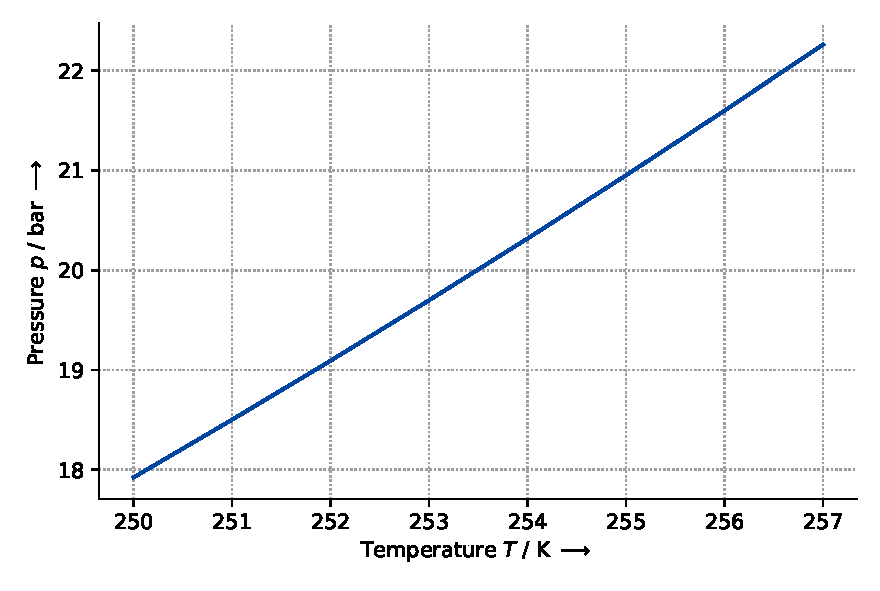
\includegraphics[height=10cm, keepaspectratio]{figs/ref/ref_CarbonDioxide_VaporPressure_EoSCubic_1.pdf}}
\end{figure}
%

\FloatBarrier
\newpage
%%%%%%%%%%%%%%%%%%%%%%%%%%%%%%%%%%%%%%%%%%%%%%%%%%%%%%%%%%%%%%%%%%%%%%%%%%%%%%%
%%%%%%%%%%%%%%%%%%%%%%%%%%%%%%%%%%%%%%%%%%%%%%%%%%%%%%%%%%%%%%%%%%%%%%%%%%%%%%%
\subsection{Vapor Pressure - EoSCubic - ID 2}
%
\begin{tabular}[l]{|lp{11.5cm}|}
\hline
\addlinespace

\textbf{Name:} & CarbonDioxide \\
\textbf{Equation:} & VaporPressure\_EoSCubic \\
\textbf{ID:} & 2 \\
\textbf{Reference:} & Lemmon, E. W.; Bell, I. H.; Huber, M. L.; McLinden, M. O. (2018): NIST Standard Reference Database 23. Reference Fluid Thermodynamic and Transport Properties-REFPROP, Version 10.0, National Institute of Standards and Technology. Online: https://www.nist.gov/srd/refprop. \\
\textbf{Comment:} & None \\

\addlinespace
\hline
\end{tabular}
\newline

\textbf{Equation and parameters:}
\newline
%
Vapor pressure $p_\mathrm{sat}$ in $\si{\pascal}$ is calculated depending on temperature $T$ in $\si{\kelvin}$ and molar volume v in $\si{\mole\per\cubic\meter}$ by using cubic equation of state. For this purpose, molar volumes of liquid and vapor phase are changed iteratively until fugacity coefficients of vapor and liquid phase are equal. Cubic equation of state is given by:
\begin{equation*}
\begin{split}
p &=& R \frac{T}{v - b} - \frac{a}{v \left(v + b\right) + b \left(v - b\right)} & \quad\text{, and} \\
a &=& 0.45724 \frac{\left(R T_\mathrm{crit} \right)^2}{p_\mathrm{crit}} \alpha & \quad\text{, and} \\
b &=& 0.07780 R \frac{T_\mathrm{crit}}{p_\mathrm{crit}} & \quad\text{, and} \\
\alpha &=& \left(1 + \kappa \left(1 - \sqrt(\nicefrac{T}{T_\mathrm{crit}}) \right) \right)^2 & \quad\text{, and} \\
\kappa &=& 0.37464 + 1.54226 \omega - 0.26992 \omega^2 & \quad\text{.}
\end{split}
\end{equation*}
%
The parameters of the equation are:
%
\begin{longtable}[l]{lll|lll}
\toprule
\addlinespace
\textbf{Par.} & \textbf{Unit} & \textbf{Value} &	\textbf{Par.} & \textbf{Unit} & \textbf{Value} \\
\addlinespace
\midrule
\endhead

\bottomrule
\endfoot
\bottomrule
\endlastfoot
\addlinespace

EoS & - & 1.000000000e+01 & $\beta_0$ & - & 0.000000000e+00 \\
$T_\mathrm{crit}$ & $\si{\kelvin}$ & 3.041300000e+02 & $\beta_1$ & - & 0.000000000e+00 \\
$p_\mathrm{crit}$ & $\si{\pascal}$ & 7.377300000e+06 & $\beta_2$ & - & 0.000000000e+00 \\
$\omega$ & - & 2.239400000e-01 & $\beta_3$ & - & 0.000000000e+00 \\
$\kappa_1$ & - & 0.000000000e+00 & & & \\

\addlinespace\end{longtable}

\textbf{Validity:}
\newline
Equation is approximately valid for $249.0785 \si{\kelvin} \leq T \leq 258.5105 \si{\kelvin}$.
\newline

\textbf{Visualization:}
%
\begin{figure}[!htp]
{\noindent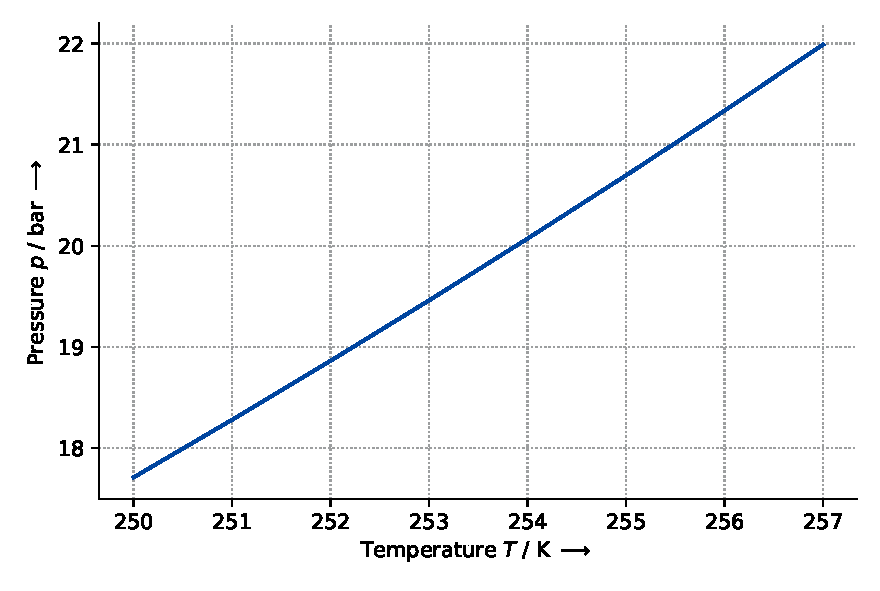
\includegraphics[height=10cm, keepaspectratio]{figs/ref/ref_CarbonDioxide_VaporPressure_EoSCubic_2.pdf}}
\end{figure}
%

\FloatBarrier
\newpage
%%%%%%%%%%%%%%%%%%%%%%%%%%%%%%%%%%%%%%%%%%%%%%%%%%%%%%%%%%%%%%%%%%%%%%%%%%%%%%%
